
\section{Optische Grundlagen}

\subsection*{Schwarzer Strahler}
Ein schwarzer Strahler ist ein idealisierter Körper, der sämtliche einfallende Strahlung absorbiert. Die aufgenommene Energie wird in Form der temperaturabhängigen Schwarzkörperstrahlung wieder ausgesandt. Die Energiedichte wird durch das Plank'sche Strahlungsgesetz beschrieben:
	\begin{align*} 
		&u(\lambda,T) = \frac{2 h c^2}{\lambda^5} \frac{1}{\exp(\frac{hc}{\lambda k_B T}) -1}\\
		&\text{u: Energiedichte}\\
		&\lambda \text{: Wellenlänge der abgestrahlten EM-Welle}\\
		&\text{T: Temperatur des schwarzen Strahlers}
	\end{align*}
Dies ergibt ein kontinuierliches Strahlungsspektrum, dessen Intensitätsmaximum bei steigender Temperatur bei schrumpfenden Wellenlängen zu finden ist. Ein Beispiel für näherungsweise schwarze Körper sind Glühlampen. Abbildung \ref{blbody} zeigt das Spektrum dreier schwarzer Strahler mit sinkenden Temperaturen. Die Lage des Intensitätsmaximums liegt im infraroten Wellenlängenbereich, weshalb Glühlampen ein "warmes" Licht abstrahlen. 
	\begin{figure}[htb]
		\centering
		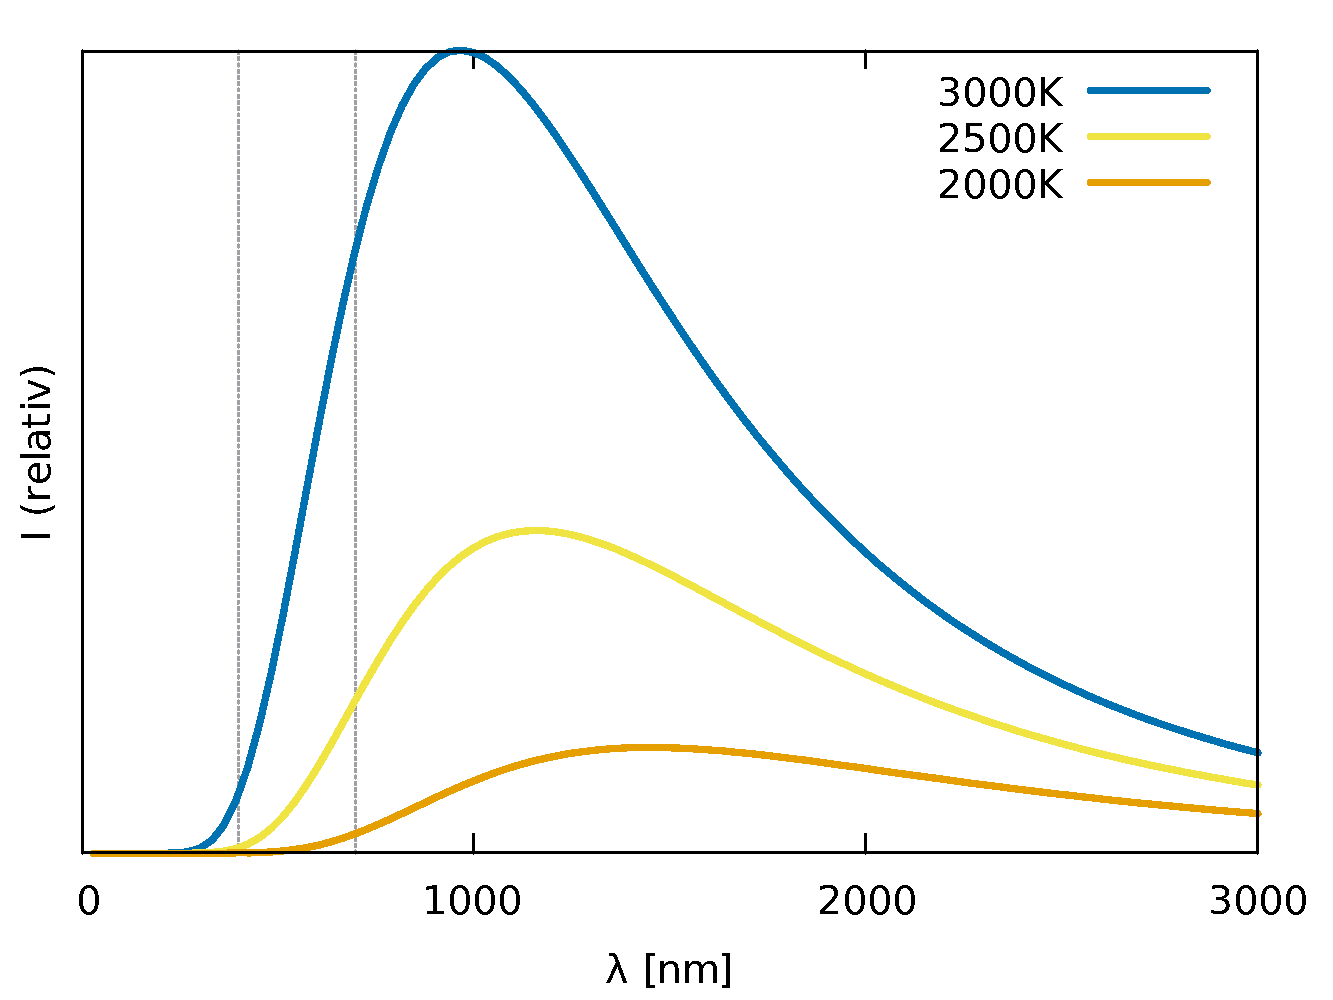
\includegraphics[width=0.6\textwidth]{Abb/blackbody.pdf}
		\caption{Spektrum schwarzer Strahler mit verschiedenen Temperaturen; sichtbarer Wellenlängenbereich markiert}
		\label{blbody}
	\end{figure}

\subsection*{Wien'sches Verschiebungsgesetz}
Das Wien'sche Verschiebungsgesetz beschreibt die Lage des Intensitätsmaximum im Strahlungsspektrum des Strahlers. Aus der Extremwertbetrachtung des Plank'schen Strahlungsgesetzes folgt, mit einigen Näherungen, das Wien'sche Verschiebungsgesetz. Somit stellt es eine Näherng des Strahlungsgesetzes dar.
\[ \lambda_{\text{max}} = \frac{\SI{2897,8}{\mu m} \, K}{T} \]
Für die drei Glühlampen in Abbildung \ref{blbody} lassen sich aus diesem Gesetz folgende Maxima errechnen:
\begin{align*}
	&\lambda_{max} (T=3000K) \approx 966 nm\\
	&\lambda_{max} (T=2500K) \approx 1160 nm\\
	&\lambda_{max} (T=2000K) \approx 1450 nm
\end{align*}
Aus dem Plot lassen sich annähernd diese Werte ablesen.
